\section{Функциональное моделирование}

В данном разделе будут предсталены временные диаграммы моделирования всей системы в целом.

В данном разделе будет рассмотрено выполнение тестовой программы, которая включает в себя все реализованные на микро-ЭВМ команды.

В ходе моделирования было решено разбить программу на две части для удобства показа на диаграммах.
Первая часть ориентирована на операции с прямой адресацией.
Она также содержит команды уловного перехода.
Вторая часть содержит команды с косвенной регистровой адресацией и команду выключения ЭВМ.

Для начала разберем программу для операций с прямой адресацией.

\subsection{Моделирование системы на основе команд с прямой адресацией}

В ходе моделирования были использованы команды, приведенные ниже.
\begin{table}[ht]
\caption{Тестовая программа для прямой адресации}
\centering
  \begin{tabular}{| >{\raggedright}m{0.45\textwidth}
                  | >{\centering}m{0.23\textwidth}
                  | >{\centering\arraybackslash}m{0.23\textwidth}|}
      \hline Мнемоническая запись команды & Первое слово & Второе слово \\
      \hline mov reg, \$mem & 4100 & 0401 \\
      \hline dec reg & 8100 & 0000 \\
      \hline push reg & 5100 & 0000 \\
      \hline pop reg & 0200 & 0000 \\
      \hline and reg, reg & 9210 & 0000 \\
      \hline ror reg, reg & b210 & 0000 \\
      \hline nand reg, reg & a120 & 0000 \\
      \hline js \$mem & e000 & 0402 \\
      \hline jmp \$mem & 6000 & 0403 \\
      \hline
  \end{tabular}
\end{table}

Для команд с прямой адресацией требуется меньше тактов на считывание и запись операндов. Но для простоты схемы все команды выполняются одинаковое количество тактов.

\begin{figure}[ht]
\centering
  \begin{subfigure}[b]{\textwidth}
    \centering
    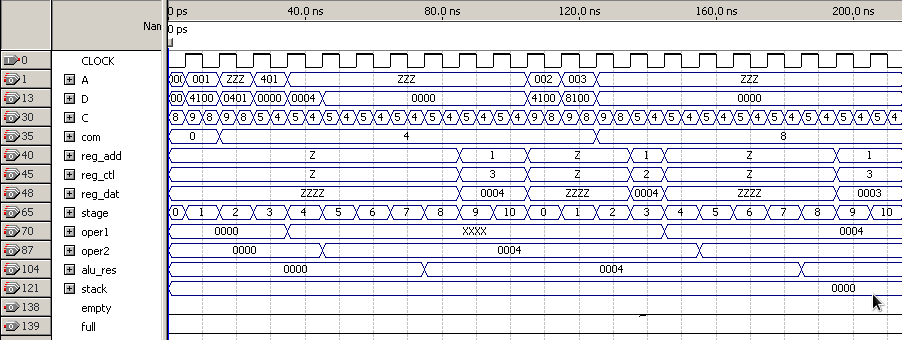
\includegraphics[scale=0.69]{pc_wave1_part1}
    \caption{}
  \end{subfigure}
    \caption{Команды mov reg, \$mem и dec reg}
\end{figure}

\begin{figure}[ht]
\centering
  \begin{subfigure}[b]{\textwidth}
    \centering
    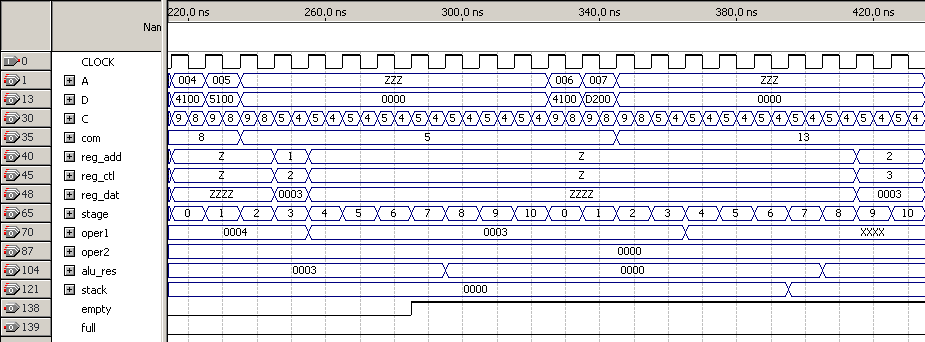
\includegraphics[scale=0.67]{pc_wave1_part2}
    \caption{}
  \end{subfigure}
    \caption{Команды push reg и pop reg}
\end{figure}

Стек вынесен в АЛУ, в блоке стека присутсвует защита от записи при заполненном стеке, а также защита от чтения при пустом стеке.
Защита от записи некорректного в операнда в регистр, при попытке достать элемент из пустого стека отсутствует.
Забота о безопасности при работе со стеком переносится на разработчиков компиляторов, для помощи им выделены сигналы full и empty, которые могут быть использованы в качестве прерываний.

\begin{figure}[ht]
\centering
  \begin{subfigure}[b]{\textwidth}
    \centering
    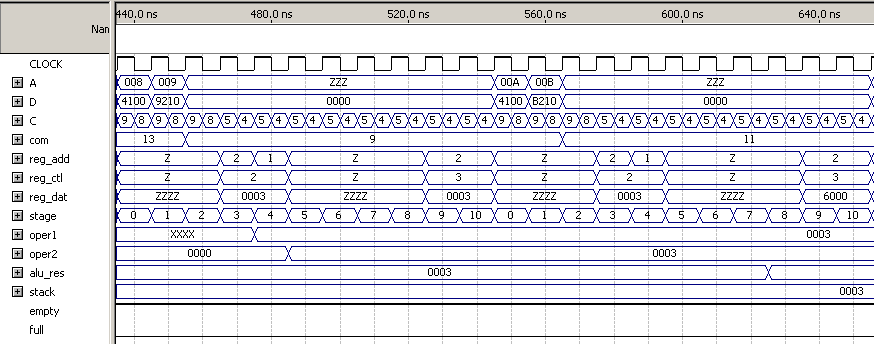
\includegraphics[scale=0.7]{pc_wave1_part3}
    \caption{}
  \end{subfigure}
    \caption{Команды and reg, reg и ror reg, reg}
\end{figure}

Команда ror работает следующим образом: первый операнд представляет собой входные данные, второй -- количество бит для сдвига вправо. В результате операнд сдвигается на заданное количестов бит вправо циклически.

\begin{figure}[ht]
\centering
  \begin{subfigure}[b]{\textwidth}
    \centering
    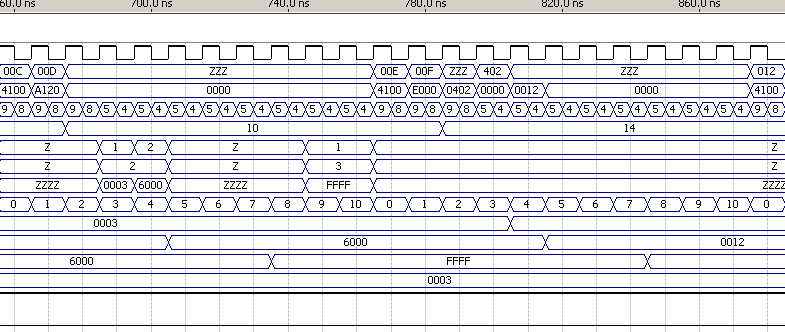
\includegraphics[scale=0.77]{pc_wave1_part4}
    \caption{}
  \end{subfigure}
    \caption{Команды nand reg, reg и js \$mem}
\end{figure}

Команда js проверяет флаг знака, устанавливаемый в АЛУ. Знак берется из старшего бита результата АЛУ, полученного при выполнении предыдущей команды.

\begin{figure}[ht]
\centering
  \begin{subfigure}[b]{\textwidth}
    \centering
    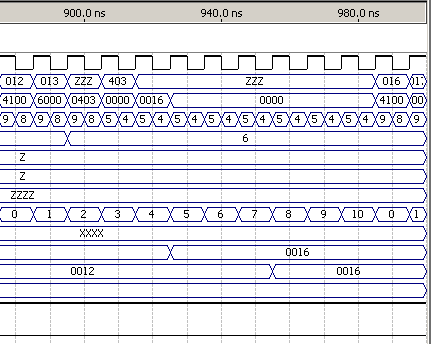
\includegraphics[scale=0.85]{pc_wave1_part5}
    \caption{}
  \end{subfigure}
    \caption{Команда jmp \$mem}
\end{figure}

Команда jmp осуществляет безусловный переход на адрес, указанный в ячейке \$mem.

\begin{figure}[ht]
\centering
  \begin{subfigure}[b]{\textwidth}
    \centering
    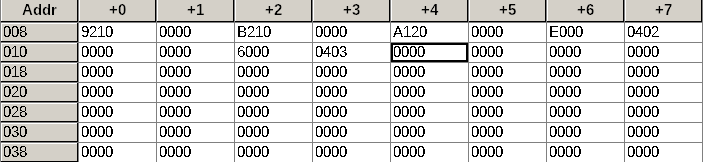
\includegraphics[scale=0.85]{rom1}
    \caption{}
  \end{subfigure}
    \caption{Файл инициализации ROM}
\end{figure}

\begin{figure}[ht]
\centering
  \begin{subfigure}[b]{\textwidth}
    \centering
    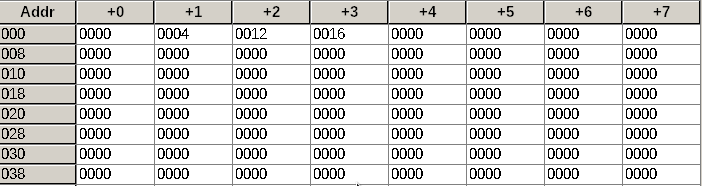
\includegraphics[scale=0.85]{ram1}
    \caption{}
  \end{subfigure}
    \caption{Файл инициализации RAM}
\end{figure}

\subsection{Моделирование системы на основе команд с косвенной адресацией}

Программа для работы с косвенной регистровой адресацией представлена ниже.
\begin{table}[ht]
\caption{Тестовая программа для косвенной адресации}
\centering
  \begin{tabular}{| >{\raggedright}m{0.45\textwidth}
                  | >{\centering}m{0.23\textwidth}
                  | >{\centering\arraybackslash}m{0.23\textwidth}|}
      \hline Мнемоническая запись команды & Первое слово & Второе слово \\
      \hline mov reg, \$mem & 4100 & 0401 \\
      \hline dec [reg] & 0010 & 0000 \\
      \hline mov reg, [reg] & 7210 & 0000 \\
      \hline and reg, [reg] & 1210 & 0000 \\
      \hline nand reg, [reg] & 2120 & 0000 \\
      \hline mov \$mem, reg & c100 & 0407 \\
      \hline ror reg, [reg] & 3220 & 0000 \\
      \hline ror reg, [reg] & 3220 & 0000 \\
      \hline hlt & f000 & 0000 \\
      \hline
  \end{tabular}
\end{table}

Рассмотрим диаграмму работы программы.

\begin{figure}[ht]
\centering
  \begin{subfigure}[b]{\textwidth}
    \centering
    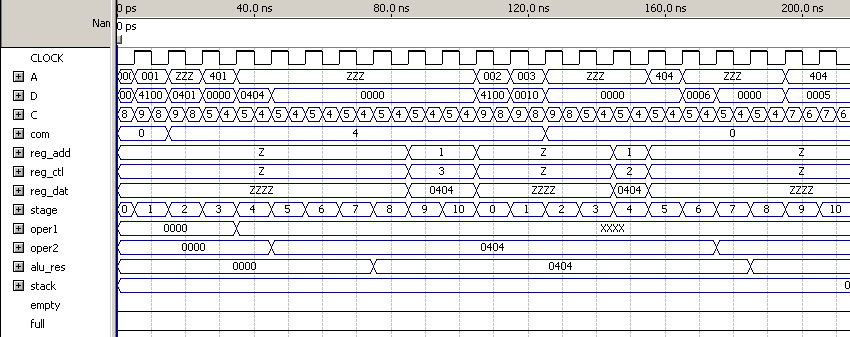
\includegraphics[scale=0.7]{pc_wave2_part1}
    \caption{}
  \end{subfigure}
    \caption{Команды mov reg, \$mem и dec[reg]}
\end{figure}

Декремент изменяет не данные в регистре, я ячейку памяти, на которую ссылается адрес в регистре, что соответствует косвенной регистровой адресации.
Для операций, подобных dec, в блок сохранения результатов был добавлен вход, который принимает адрес памяти, по которому хранится операнд. Это позволяет пересылку данных в ячейки, адресуемые с помощью косвенной регистровой адресации.

\begin{figure}[ht]
\centering
  \begin{subfigure}[b]{\textwidth}
    \centering
    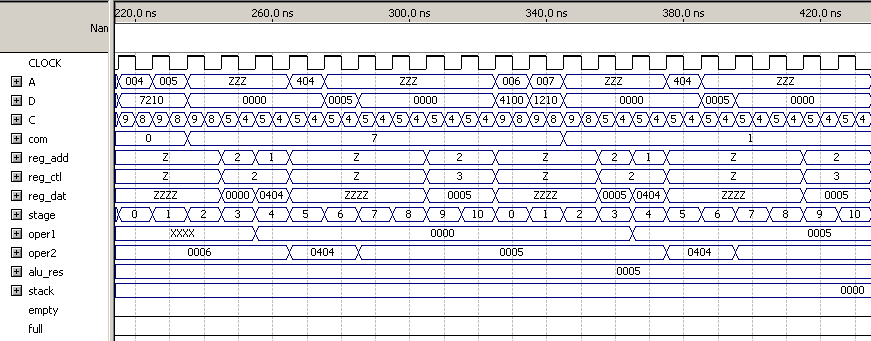
\includegraphics[scale=0.68]{pc_wave2_part2}
    \caption{}
  \end{subfigure}
    \caption{Команды mov reg, [reg] и and reg, [reg]}
\end{figure}

Во время этапа выборки операндов(такты 3-6) происходит чтение адреса из регистра, обращение к ячейки памяти по этому адресу и сохранение значения в промежуточный регистр.

\begin{figure}[ht]
\centering
  \begin{subfigure}[b]{\textwidth}
    \centering
    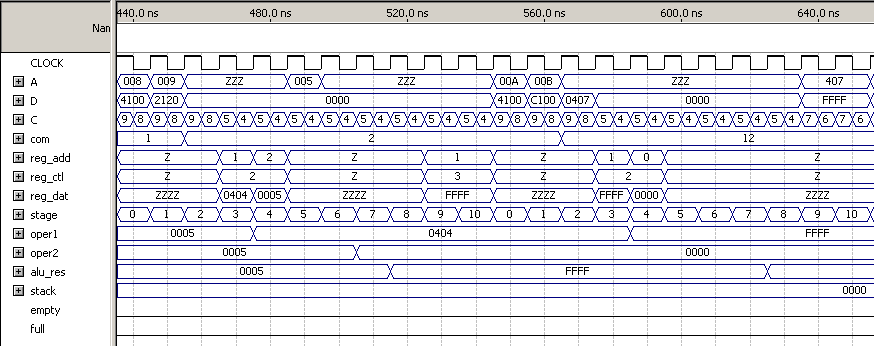
\includegraphics[scale=0.68]{pc_wave2_part3}
    \caption{}
  \end{subfigure}
    \caption{Команды nand reg, [reg] и mov \$mem, reg}
\end{figure}

Все операнды попадают в АЛУ и дальше проходит лишь один из них. Данное решение оказалось не слишком удачным и пришлось задействовать дополнительный вход в блоке сохранения результата, из-за того, что через АЛУ по умолчанию проходят лишь первые операнды(полученные в результате прямой и прямой регистровой адресации).

\begin{figure}[ht]
\centering
  \begin{subfigure}[b]{\textwidth}
    \centering
    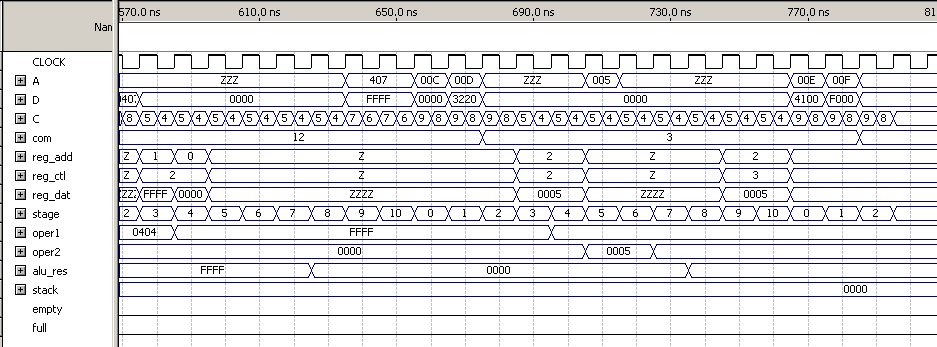
\includegraphics[scale=0.65]{pc_wave2_part4}
    \caption{}
  \end{subfigure}
    \caption{Команды ror reg, [reg] и hlt}
\end{figure}

В ходе команды hlt произошло отделение системы от синхроимпульса, тем самым была произведена остановка всей системы.

Содержимое ROM файла с программой, содержимое RAM начале работы программы, а также содержимое RAM после окончания работы программы представлено на рисунках ниже.

\begin{figure}[ht]
\centering
  \begin{subfigure}[b]{\textwidth}
    \centering
    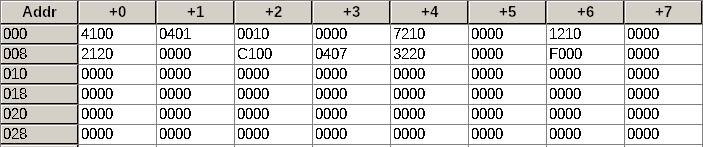
\includegraphics[scale=0.8]{rom2}
    \caption{}
  \end{subfigure}
    \caption{Файл инициализации ROM"}
\end{figure}

\begin{figure}[ht]
\centering
  \begin{subfigure}[b]{\textwidth}
    \centering
    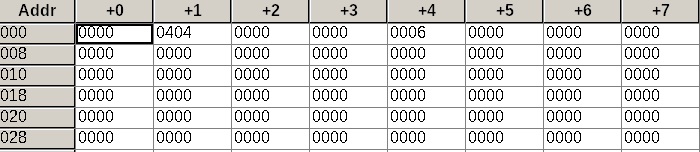
\includegraphics[scale=0.8]{ram21}
    \caption{}
  \end{subfigure}
    \caption{Содержимое файла инициализации RAM}
\end{figure}

\begin{figure}[ht]
\centering
  \begin{subfigure}[b]{\textwidth}
    \centering
    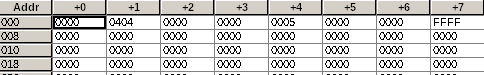
\includegraphics[scale=1.15]{ram22}
    \caption{}
  \end{subfigure}
    \caption{Содержимое RAM после моделирования}
\end{figure}
